\chapter{非平衡载流子}

\section{非平衡载流子的注入和复合}

处于热平衡下的载流子浓度称为\textbf{平衡载流子浓度}。一般用$n_0$和$p_0$分别表示平衡电子浓度和空穴浓度。非简并条件下,其乘积满足关系:
\begin{equation}
    n_0p_0=N_vN_c\exp{\left(-\frac{E_g}{k_0T}\right)}=n_i^2
\end{equation}

对半导体施加外界作用,破坏热平衡条件,使半导体处于与热平衡偏离的状态,称为\textbf{非平衡状态}。处于非平衡状态的半导体,其载流子浓度浓度不再为$n_0$和$p_0$,而会多出一部分。比平衡状态多出的载流子称为\textbf{非平衡载流子}或\textbf{过剩载流子}。

一定温度下,n型半导体中,$n_0\gg p_0$,用适当波长的光照射半导体,且光子能量大于半导体的禁带宽度,则光子可以将价带电子激发到导带上,形成电子-空穴对,导带比平衡时多出$\Delta n$的电子,即\textbf{非平衡电子},称为\textbf{非平衡多数载流子(多子)};价带多出$\Delta p$的空穴,即\textbf{非平衡空穴},称为\textbf{非平衡少数载流子(少子)}。这种通过光照产生非平衡载流子的方法,称为非平衡载流子的\textbf{光注入}。光注入时有:
\begin{equation}
    \Delta n=\Delta p
\end{equation}

一般情况下,注入的非平衡载流子浓度比平衡时的多数载流子浓度小得多。对上述情况,有:
\begin{equation}
    \Delta n\ll n_0,\quad \Delta p\ll n_0
\end{equation}
满足此条件的注入称为\textbf{小注入}。在小注入条件下,非平衡少子的浓度也可以比平衡少子的浓度大得多,如上例中有$\Delta p\gg p_0$。非平衡少子常常会起决定性作用。通常所说的非平衡载流子都指非平衡少子。

光注入导致半导体的电导率增大。附加电导率为:
\begin{equation}
    \Delta \sigma=\Delta nq\mu_n+\Delta pq\mu_p=\Delta pq(\mu_n+\mu_p)
\end{equation}

设半导体平衡电导率为$\sigma_0$,光照引起附加电导率$\Delta \sigma$,小注入条件下$\sigma_0+\Delta \sigma\approx\sigma_0$,电阻率改变:
\begin{equation}
    \Delta\rho=\frac{1}{\sigma}-\frac{1}{\sigma_0}=\frac{1}{\sigma_0+\Delta\sigma}-\frac{1}{\sigma_0}=-\frac{\Delta\sigma}{(\sigma_0+\Delta\sigma)\sigma_0}\approx-\frac{\Delta\sigma}{\sigma_0^2}
\end{equation}
半导体电阻改变:
\begin{equation}
    \Delta r=\Delta\rho\frac{l}{s}\approx-\frac{l}{s\sigma_0^2}\Delta\sigma
\end{equation}
$l,\ s$为半导体的长度和截面积。因此$\Delta r\propto \Delta \sigma$。半导体通电时,由于电势差$\Delta V=I\Delta r$,故$\Delta V\propto\Delta\sigma$,因此$\Delta V\propto\Delta p$:
\begin{equation}
    \Delta V=-\frac{l}{s\sigma^2}Iq(\mu_n+\mu_p)\Delta p
\end{equation}

\section{非平衡载流子的寿命}

小注入时,$\Delta V$的变化反映了$\Delta p$的变化。光照停止后,$\Delta p$随时间按指数减小。非平衡载流子的平均生存时间称为载流子的\textbf{寿命},用$\tau$表示(上章有个叫平均自由时间的物理量也记成$\tau$来
着
\includegraphics[width=4em, align=c]{idiot.jpg})。由于非平衡少子相比多子更占主导地位,因此非平衡载流子的寿命常称为\textbf{少子的寿命}。显然$\D \frac{1}{\tau}$是单位时间内非平衡载流子的复合概率。\vspace{1ex}
通常将单位时间单位体积内净复合消失的电子-空穴对数称为非平衡载流子的\textbf{复合率}。显然,$\D \frac{\Delta p}{\tau}$就是复合率。

一束光在一块n型半导体内均匀产生非平衡载流子$\Delta n$和$\Delta p$。$t=0$时光照停止,\vspace{1ex}
$\Delta p$会随时间变化,单位时间内浓度减小$\D -\frac{\mathrm{d}\Delta p(t)}{\mathrm{d}t}$,减小是由电子-空穴对的复合引起的,应当等于非平衡载流子的复合率:
\begin{equation}
    \frac{\mathrm{d}\Delta p(t)}{\mathrm{d}t}=-\frac{\Delta p}{\tau}
\end{equation}
寿命$\tau$在小注入条件下是个恒量,与$\Delta p(t)$无关。解这个微分方程:
\begin{equation}
    \Delta p(t)=C\mathrm{e}^{-\frac{t}{\tau}}
\end{equation}
设$t=0$时刻停止光照时少子浓度$\Delta p(0)=\Delta p_0$,作为边界条件代入微分方程,解得系数为$C=\Delta p_0$,故:
\begin{equation}
    \Delta p(t)=\Delta p_0\mathrm{e}^{-\frac{t}{\tau}}
\end{equation}
即非平衡载流子浓度随时间按指数衰减。

\section{准费米能级}

热平衡下的半导体中电子和空穴具有统一的费米能级。非简并条件下:
\begin{equation}
    n_0=N_c\exp{\left(-\frac{E_c-E_F}{k_0T}\right)},\quad p_0=N_v\exp{\left(-\frac{E_F-E_v}{k_0T}\right)}\label{eq:chap-5-equilibrium-distribute}
\end{equation}
外界影响下破坏了热平衡,非平衡态的半导体不再具有统一的费米能级。我们认为价带和导带中的电子与空穴各自处于平衡状态,但价带与导带之间不处于平衡态。因此可以分别引入\textbf{导带费米能级}和\textbf{价带费米能级},均为\textbf{局部费米能级},称为\textbf{准费米能级}。导带费米能级也称为\textbf{电子准费米能级},用$E_{Fn}$表示,价带准费米能级也称为\textbf{空穴准费米能级},用$E_{Fp}$表示。

非平衡下的载流子浓度可以用与平衡载流子浓度类似公式表达:
\begin{equation}
    n=N_c\exp{\left(-\frac{E_c-E_{Fn}}{k_0T}\right)},\quad p=N_v\exp{\left(-\frac{E_{Fp}-E_v}{k_0T}\right)}
\end{equation}
上式适用的条件与平衡态载流子相同,即$E_{Fn}$和$E_{Fp}$不能进入导带或价带。参考\autoref{eq:chap-5-equilibrium-distribute},可以推导出$n$与$n_0$,$p$与$p_0$的关系:
\begin{align}
&
\begin{aligned}
    n&=N_c\exp{\left(-\frac{E_c-E_{Fn}}{k_0T}\right)}\\
    &=N_c\exp{\left(-\frac{E_c-E_{F}}{k_0T}\right)}\exp{\left(\frac{E_{Fn}-E_F}{k_0T}\right)}\\
    &=n_0\exp{\left(\frac{E_{Fn}-E_F}{k_0T}\right)}
\end{aligned}
\\
&
\begin{aligned}
    p&=N_v\exp{\left(-\frac{E_{Fp}-E_v}{k_0T}\right)}\\
    &=N_v\exp{\left(-\frac{E_{F}-E_v}{k_0T}\right)}\exp{\left(\frac{E_F-E_{Fp}}{k_0T}\right)}\\
    &=p_0\exp{\left(\frac{E_F-E_{Fp}}{k_0T}\right)}
\end{aligned}
\end{align}
由
\begin{equation}
    n_0=n_i\exp{\left(-\frac{E_i-E_F}{k_0T}\right)},\quad p_0=n_i\exp{\left(\frac{E_i-E_F}{k_0T}\right)}
\end{equation}
进一步推导:
\begin{align}
&
    \begin{aligned}
        n&=n_0\exp{\left(\frac{E_{Fn}-E_F}{k_0T}\right)}\\
        &=n_i\exp{\left(-\frac{E_i-E_F}{k_0T}\right)}\exp{\left(\frac{E_{Fn}-E_F}{k_0T}\right)}\\
        &=n_i\exp{\left(\frac{E_{Fn}-E_i}{k_0T}\right)}
    \end{aligned}
    \\
&
    \begin{aligned}
        p&=p_0\exp{\left(\frac{E_F-E_{Fp}}{k_0T}\right)}\\
        &=n_i\exp{\left(\frac{E_i-E_F}{k_0T}\right)}\exp{\left(\frac{E_F-E_{Fp}}{k_0T}\right)}\\
        &=n_i\exp{\left(\frac{E_i-E_{Fp}}{k_0T}\right)}
    \end{aligned}
\end{align}
电子与空穴浓度的乘积:
\begin{equation}
    np=n_0p_0\exp{\left(\frac{E_{Fn}-E_{Fp}}{k_0T}\right)}
\end{equation}

\section{复合理论}

\subsection{载流子复合的分类}

半导体\textbf{复合}的过程即半导体\textbf{由非平衡态向平衡态过渡}的过程。半导体的复合过程大致可分为:
\begin{enumerate}
    \item 直接复合:电子在导带与价带间直接跃迁,实现电子与空穴的复合。
    \item 间接复合:电子与空穴通过禁带能级复合。简介复合按照发生位置可以分为\textbf{体内复合}和\textbf{表面复合}。
\end{enumerate}
载流子复合时会放出多余能量,放出能量的方法有:
\begin{enumerate}
    \item 发射光子:伴随复合,伴有发光现象,称为\textbf{发光复合}或\textbf{辐射复合}。
    \item 发射声子:载流子将多余能量传递给晶格,加强晶格振动。
    \item 能量给予其他载流子,增大动能,称为\textbf{俄歇(Auger)复合}。
\end{enumerate}

\subsection{直接复合}

半导体中同时存在着载流子的\textbf{产生}和和\textbf{复合}两个过程。单位时间内产生的电子-空穴对数称为\textbf{产生率},记为$G$,复合的电子-空穴对数称为\textbf{复合率},记为$R$。

$n,\ p$分别为电子和空穴浓度。单位体积,单位时间里,每个电子都有概率和空穴复合,复合概率与空穴浓度成正比,即每个电子复合的概率为$rp$,$r$是比例系数。每个电子复合概率再乘以电子浓度就是全部电子的复合率,即:
\begin{equation}
    R=rnp
\end{equation}
比例系数$r$称为\textbf{电子-空穴复合概率},它代表着所有电子和空穴复合概率的平均值。

载流子受激发的概率不受载流子浓度的影响,产生率在所有非简并情况下是相同的,即$G$仅与温度有关,和$n,\ p$无关。

热平衡时,产生率等于复合率:$P=G$,此时$n=n_0,\ p=p_0$,因此得到$G$与$r$的关系:
\begin{equation}
    G=P=rn_0p_0=rn_i^2
\end{equation}
复合率减产生率即非平衡载流子的净复合率,得到净复合率$U_d$为:
\begin{equation}
    U_d=R-G=rnp-rn_i^2=r(np-n_i^2)
\end{equation}
代入关系$n=n_0+\Delta n,\ p=p_0+\Delta p,\ \Delta n=\Delta p$,得:
\begin{align}
    U_d&=r[(n_0+\Delta n)(p_0+\Delta p)-n_0p_0]\notag\\
    &=r(n_0\Delta p+p_0\Delta p+\Delta p^2)\notag\\
    &=r(n_0+p_0)\Delta p+r\Delta p^2
\end{align}
由于净复合率和载流子寿命存在关系:
\begin{equation}
    U_d=\frac{\Delta p}{\tau}
\end{equation}
得载流子寿命:
\begin{equation}
    \tau=\frac{\Delta p}{U_d}=\frac{1}{r[(n_0+p_0)+\Delta p]}\label{eq:chap-5-direct-recombination-lifetime}
\end{equation}
可见寿命$\tau$不仅与平衡载流子浓度有关,也与非平衡载流子浓度有关。

在小注入条件下,$\Delta p\ll (n_0+p_0)$,\autoref{eq:chap-5-direct-recombination-lifetime}近似为:
\begin{equation}
    \tau\approx\frac{1}{r(n_0+p_0)}
\end{equation}
对n型材料,$n_0\gg p_0$,上式近似有
\begin{equation}
    \tau\approx\frac{1}{rn_0}
\end{equation}
寿命与非平衡载流子无关,与多数载流子成反比。

当$\Delta p\gg n_0+p_0$时,\autoref{eq:chap-5-direct-recombination-lifetime}近似有:
\begin{equation}
    \tau\approx\frac{1}{r\Delta p}
\end{equation}
此时寿命与非平衡载流子成反比。

\subsection{间接复合}

半导体中的杂质和缺陷会促进非平衡载流子的复合过程,这些促进复合的杂质和缺陷称为\textbf{复合中心}。间接复合即非平衡载流子通过复合中心的复合。

记复合中心能级$E_t$,如\autoref{fig:indirect-recombination-process},能级$E_t$上的间接复合具有四个过程:
\begin{enumerate}[(1)]
    \item 俘获电子:复合中心能级$E_t$从导带俘获电子。
    \item 发射电子:复合中心能级$E_t$上的电子被激发到导带。
    \item 俘获空穴:电子由复合中心能级$E_t$落入价带,与空穴复合,可以看成复合中心能级$E_t$从价带俘获一个电子。
    \item 发射空穴:价带电子激发到复合中心能级$E_t$,可以看出复合中心能级$E_t$向价带发射一个空穴。
\end{enumerate}

\begin{figure}[ht]
    \centering
\tikzset{every picture/.style={line width=0.75pt}} %set default line width to 0.75pt        

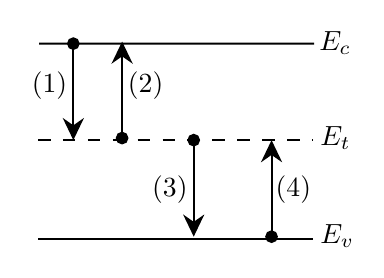
\begin{tikzpicture}[x=0.75pt,y=0.75pt,yscale=-1,xscale=1]
%uncomment if require: \path (0,300); %set diagram left start at 0, and has height of 300

%Straight Lines [id:da20064609469527683] 
\draw    (120.67,31.08) -- (137.17,31.09) -- (253.17,31.1) ;
%Straight Lines [id:da19330925404980026] 
\draw  [dash pattern={on 4.5pt off 4.5pt}]  (120.17,77.5) -- (252.67,77.5) ;
%Straight Lines [id:da5528060898844296] 
\draw    (120.17,125) -- (252.67,125) ;
%Shape: Circle [id:dp32843318610089023] 
\draw  [fill={rgb, 255:red, 0; green, 0; blue, 0 }  ,fill opacity=1 ] (134.63,31.09) .. controls (134.63,32.49) and (135.76,33.63) .. (137.17,33.63) .. controls (138.57,33.63) and (139.71,32.49) .. (139.71,31.09) .. controls (139.71,29.68) and (138.57,28.54) .. (137.17,28.54) .. controls (135.76,28.54) and (134.63,29.68) .. (134.63,31.09) -- cycle ;
%Straight Lines [id:da48904866335535435] 
\draw    (137.17,31.09) -- (137.17,74.58) ;
\draw [shift={(137.17,77.58)}, rotate = 270] [fill={rgb, 255:red, 0; green, 0; blue, 0 }  ][line width=0.08]  [draw opacity=0] (10.72,-5.15) -- (0,0) -- (10.72,5.15) -- (7.12,0) -- cycle    ;
%Straight Lines [id:da7345813081514647] 
\draw    (160.67,33.09) -- (160.67,76.58) ;
\draw [shift={(160.67,30.09)}, rotate = 90] [fill={rgb, 255:red, 0; green, 0; blue, 0 }  ][line width=0.08]  [draw opacity=0] (10.72,-5.15) -- (0,0) -- (10.72,5.15) -- (7.12,0) -- cycle    ;
%Shape: Circle [id:dp42146991706121617] 
\draw  [fill={rgb, 255:red, 0; green, 0; blue, 0 }  ,fill opacity=1 ] (158.12,76.58) .. controls (158.12,77.99) and (159.26,79.13) .. (160.67,79.13) .. controls (162.07,79.13) and (163.21,77.99) .. (163.21,76.58) .. controls (163.21,75.18) and (162.07,74.04) .. (160.67,74.04) .. controls (159.26,74.04) and (158.12,75.18) .. (158.12,76.58) -- cycle ;
%Straight Lines [id:da21853964923058133] 
\draw    (195.17,77.59) -- (195.17,121.08) ;
\draw [shift={(195.17,124.08)}, rotate = 270] [fill={rgb, 255:red, 0; green, 0; blue, 0 }  ][line width=0.08]  [draw opacity=0] (10.72,-5.15) -- (0,0) -- (10.72,5.15) -- (7.12,0) -- cycle    ;
%Shape: Circle [id:dp8914894742891817] 
\draw  [fill={rgb, 255:red, 0; green, 0; blue, 0 }  ,fill opacity=1 ] (192.63,77.59) .. controls (192.63,78.99) and (193.76,80.13) .. (195.17,80.13) .. controls (196.57,80.13) and (197.71,78.99) .. (197.71,77.59) .. controls (197.71,76.18) and (196.57,75.04) .. (195.17,75.04) .. controls (193.76,75.04) and (192.63,76.18) .. (192.63,77.59) -- cycle ;
%Straight Lines [id:da2456794806958813] 
\draw    (232.67,80.59) -- (232.67,124.08) ;
\draw [shift={(232.67,77.59)}, rotate = 90] [fill={rgb, 255:red, 0; green, 0; blue, 0 }  ][line width=0.08]  [draw opacity=0] (10.72,-5.15) -- (0,0) -- (10.72,5.15) -- (7.12,0) -- cycle    ;
%Shape: Circle [id:dp5273521015953397] 
\draw  [fill={rgb, 255:red, 0; green, 0; blue, 0 }  ,fill opacity=1 ] (230.12,124.08) .. controls (230.12,125.49) and (231.26,126.63) .. (232.67,126.63) .. controls (234.07,126.63) and (235.21,125.49) .. (235.21,124.08) .. controls (235.21,122.68) and (234.07,121.54) .. (232.67,121.54) .. controls (231.26,121.54) and (230.12,122.68) .. (230.12,124.08) -- cycle ;

% Text Node
\draw (115.67,43) node [anchor=north west][inner sep=0.75pt]   [align=left] {(1)};
% Text Node
\draw (162,43) node [anchor=north west][inner sep=0.75pt]   [align=left] {(2)};
% Text Node
\draw (173.67,93) node [anchor=north west][inner sep=0.75pt]   [align=left] {(3)};
% Text Node
\draw (233.17,93) node [anchor=north west][inner sep=0.75pt]   [align=left] {(4)};
% Text Node
\draw (254.67,116.9) node [anchor=north west][inner sep=0.75pt]    {$E_{v}$};
% Text Node
\draw (254.17,23.9) node [anchor=north west][inner sep=0.75pt]    {$E_{c}$};
% Text Node
\draw (254.67,69.4) node [anchor=north west][inner sep=0.75pt]    {$E_{t}$};
\end{tikzpicture}
    \caption{复合中心能级$E_t$的四个间接复合过程}
    \label{fig:indirect-recombination-process}
\end{figure}

$n$和$p$分别为导带电子和价带空穴浓度,设复合中心浓度为$N_t$,复合中心能级上的电子浓度为$n_t$,则未被电子占据的复合中心浓度为$N_t-n_t$。

(1) 过程中,我们把单位体积、单位时间内内复合中心俘获的电子数称为\textbf{电子俘获率}。电子俘获率与导带电子浓度$n$和未被占据的复合中心浓度$(N_t-n_t)$成正比:
\begin{equation}
    \text{电子俘获率}=r_nn(N_t-n_t)
\end{equation}
比例系数$r_n$是\textbf{电子俘获系数},反映了复合中心平均俘获电子能力的大小。

(2) 过程是 (1) 过程的逆过程。我们用电子产生率表示单位时间、单位体积向导带发射的电子数。只有已被占据的复合中心才能向导带发射电子,导带近似认为是空的,因此电子产生率与$n_t$成正比,和$n$无关:
\begin{equation}
    \text{电子产生率}=s_-n_t
\end{equation}
$s_-$称为\textbf{电子激发概率},仅与温度有关。

平衡时,(1) 过程和 (2) 过程相互抵消,电子产生率等于电子俘获率:
\begin{equation}
    r_nn_0(N_t-n_{t0})=s_-n_{t0}\label{eq:chap-5-equilibrium-indirect-recombination-electron-equation}
\end{equation}
$n_0$和$n_{t0}$分别为平衡时导带和复合中心能级上的电子浓度。计算$n_{t0}$时,我们忽略分布函数中的简并因子:
\begin{equation}
    n_{t0}=N_tf(E_t)=N_t\frac{1}{\D 1+\exp{\left(\frac{E_t-E_F}{k_0T}\right)}}
\end{equation}
非简并条件下:
\begin{equation}
    n_0=N_c\exp{\left(\frac{E_F-E_c}{k_0T}\right)}
\end{equation}
将$n_0$和$n_{t0}$表达式代入\autoref{eq:chap-5-equilibrium-indirect-recombination-electron-equation}:
\begin{align}
    s_-N_t\frac{1}{\D 1+\exp{\left(\frac{E_t-E_F}{k_0T}\right)}}&=r_nN_c\exp{\left(\frac{E_F-E_c}{k_0T}\right)}N_t\left[1-\left(\frac{1}{\D 1+\exp{\left(\frac{E_t-E_F}{k_0T}\right)}}\right)\right]\notag\\
    \Longrightarrow s_-&=r_nN_c\exp{\left(\frac{E_F-E_c}{k_0T}\right)}\exp{\left(\frac{E_t-E_F}{k_0T}\right)}\notag\\
    \Longrightarrow s_-&=r_nN_c\exp{\left(\frac{E_t-E_c}{k_0T}\right)}
\end{align}
记:
\begin{equation}
    n_1=N_c\exp{\left(\frac{E_t-E_c}{k_0T}\right)}
\end{equation}
$n_1$等于费米能级与复合中心能级重合时导带电子平均浓度。代入:
\begin{equation}
    s_-=r_nN_c\exp{\left(\frac{E_t-E_c}{k_0T}\right)}=r_nn_1
\end{equation}
将上式代入电子产生率中:
\begin{equation}
    \text{电子产生率}=r_nn_1n_t
\end{equation}

(3) 过程中,空穴俘获率与$n_t$和$p$成正比:
\begin{equation}
    \text{空穴俘获率}=r_ppn_t
\end{equation}
$r_p$称为\textbf{空穴俘获系数},反映复合中心平均俘获空穴的能力.

(4) 过程是 (3) 的逆过程类似上文讨论,有:
\begin{equation}
    \text{空穴产生率}=s_+(N_t-n_t)
\end{equation}
$s_+$为\textbf{空穴激发概率}。

平衡时,(3) 和 (4) 过程相互抵消:
\begin{equation}
    s_+(N_t-n_{t0})=r_pp_0n_{t0}
\end{equation}
代入平衡时$p_0$和$n_{t0}$值,得:
\begin{equation}
    s_+=r_pp_1
\end{equation}
其中
\begin{equation}
    p_1=N_v\exp{\left(-\frac{E_t-E_v}{k_0T}\right)}
\end{equation}
$p_1$等于费米能级和复合中心能级重合时价带的平衡空穴浓度。

将$s_+$表达式代入空穴产生率,得:
\begin{equation}
    \text{空穴产生率}=r_pp_1(N_t-n_t)
\end{equation}




